\subsection{Interacting Method}

제안하는 시스템은 컴퓨팅 인터페이스에 익숙하지 않은 작업 인부들도 직관적으로 3차원 정보에 접근하고 작업을 처리할 수 있도록 하기 위하여 펜과 finger를 사용하여 직관적인 인터페이스를 제공하도록 설계하였다. 이러한 방법은 기존의 3D 모델 처리를 위한 Interactive Tabletop 연구들\cite{brandl_combining_2008, lopes_combining_2011}에서 많이 연구되었으며, 본 논문에서는 이러한 방법을 3차원 공간으로 확장하였다. 특히 \cite{guiard_asymmetric_1987}에서는 양 손의 역할에 대하여 비대칭적인 관계가 있음을 증명하였다. 이에 제안하는 시스템에서도 dominant hand(DH)로 이루어지는 펜 인터렉션과 non-dominant hand(NDH)로 이루어지는 Finger 인터렉션을 구분하여 설계하였다.

\begin{table}[h!]
  \centering
  \begin{tabular}{|p{10mm}|p{30mm}|p{30mm}|}		% l, c, r을 쓰면 두 행이 되지 않는다
%  \begin{tabular}{|c|c|c|}
    \hline
    \tabhead{} &
    \multicolumn{1}{|p{0.3\columnwidth}|}{\centering\tabhead{3D In-Air}} &
    \multicolumn{1}{|p{0.3\columnwidth}|}{\centering\tabhead{2D Surface}} \\
    \hline
    \centering{Finger\\(NDH)} & 3D model browsing & calculate dimension \\
    \hline
    \centering{Pen\\(DH)} & annotating/editing to 3D entity in the 3D model & annotating/editing to 2D entity in the floor plan \\
    \hline
  \end{tabular}
  \caption{Interaction design to bimanual pen and finger interaction}
  \label{tab:table1}
\end{table}

\textit{Mobile Personal Workspace에서는 스마트 폰을 이용하여 상호작용을 제공한다. 모바일 폰 기반의 상호작용은 크게 두 가지 방법을 지원한다. 먼저 폰 자체의 Pose를 이용하여 Shared Workspace의 컨텐츠를 회전하거나 조작할 수 있으며, 이는 Co-location에서 회의하거나 할 때 Shared Workspace의 Interaction을 확장하여 준다. 또한, 터치 기반의 상호작용으로, 멀티터치를 이용하여 객체를 회전, 스케일 변환하거나 싱글 터치로 객체를 선택하고 Drag를 이용하여 이동시키거나 변경할 수 있다. }


\subsection{3D Model Manipulation}

\begin{figure*}[!ht]
	\centering
        \begin{subfigure}[b]{0.32\textwidth}
	        \centering
                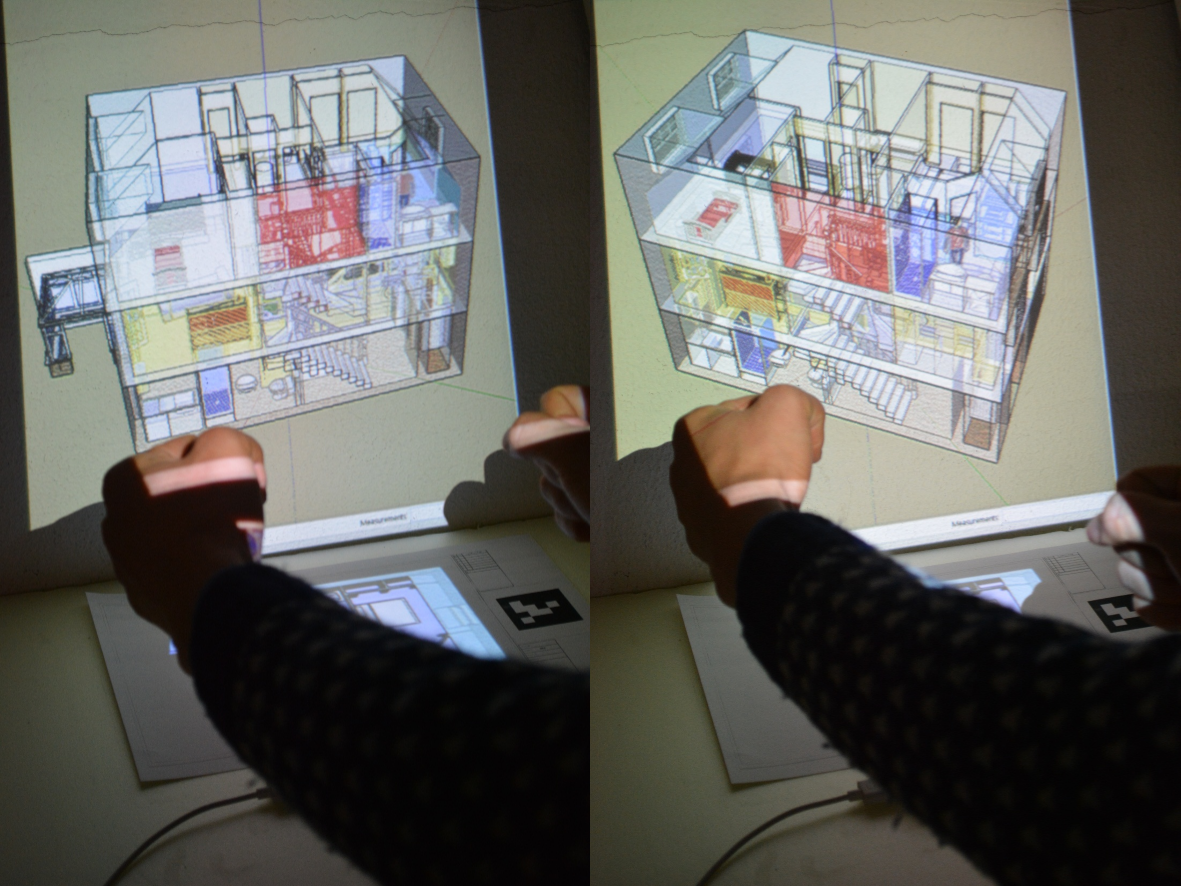
\includegraphics[width=\textwidth]{4-Interaction_Design/3d_rotate}
                \caption{Rotating the Model}
                \label{fig:rotate}
        \end{subfigure}%
        \hfill
        \begin{subfigure}[b]{0.32\textwidth}
            \centering
            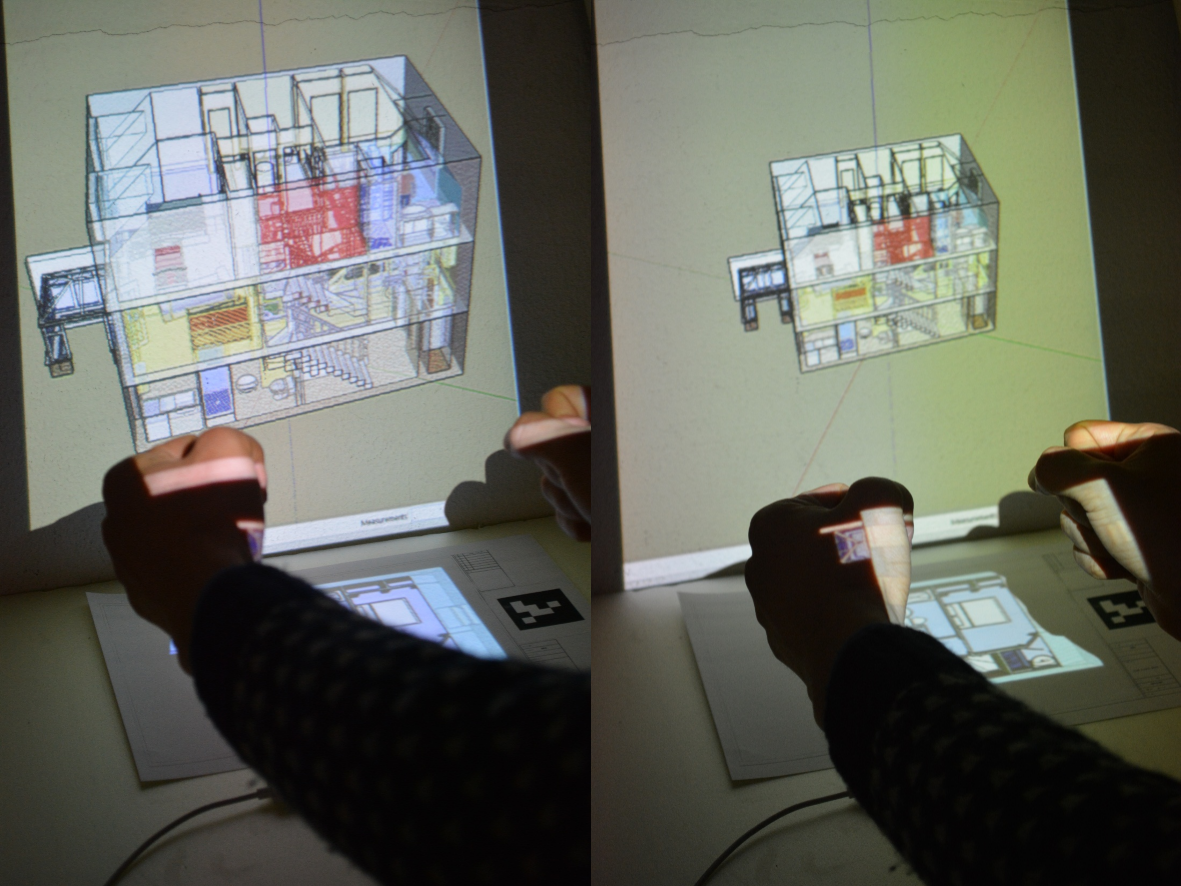
\includegraphics[width=\textwidth]{4-Interaction_Design/3d_scale_two_hand}
                \caption{Scaling by Two Hand Gesture}
                \label{fig:scale_two_hand}
        \end{subfigure}
        \hfill
        \begin{subfigure}[b]{0.32\textwidth}
            \centering
            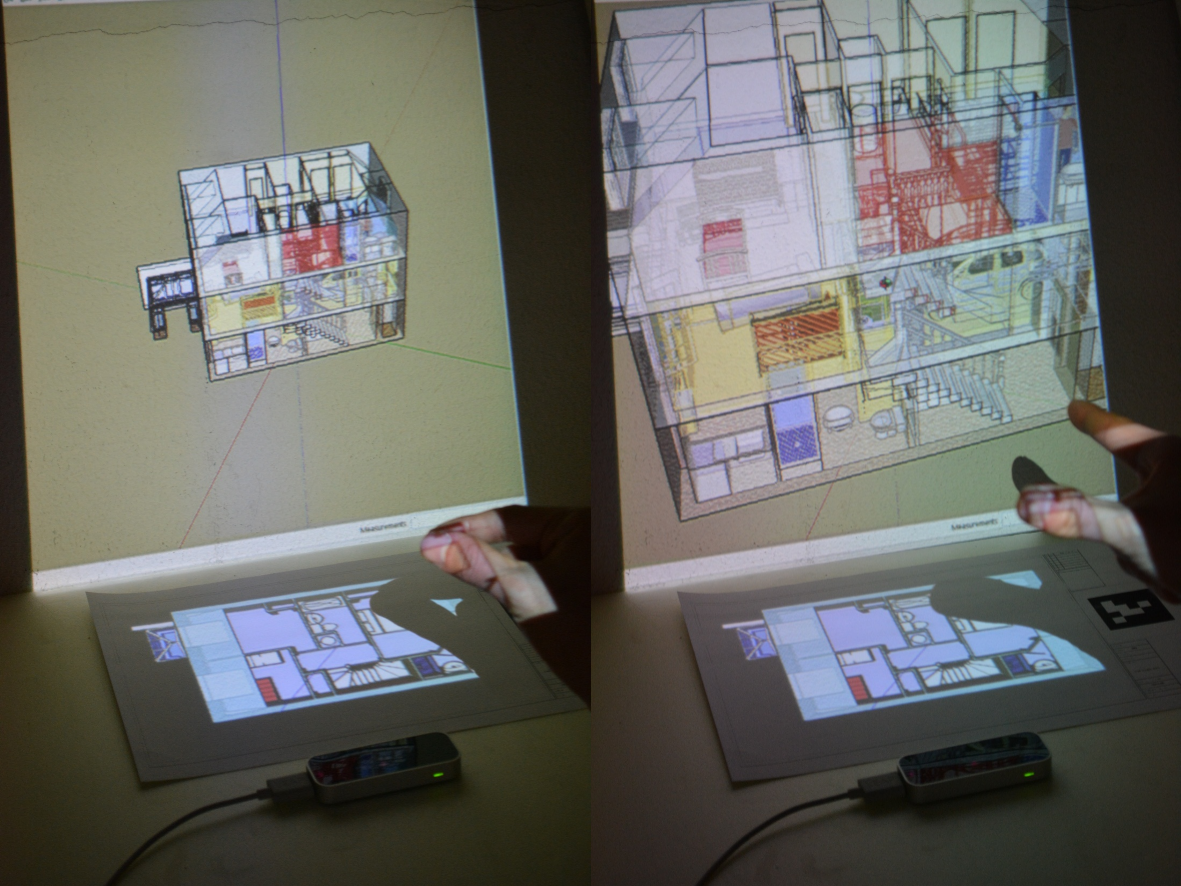
\includegraphics[width=\textwidth]{4-Interaction_Design/3d_scale_one_hand}
                \caption{Scaling by One Hand Gesture}
                \label{fig:scale_pinch}
        \end{subfigure}
	\caption{3D Manipulation}
    \label{fig:3d_mani}
\end{figure*}


설계도는 3차원의 현실 세계를 2차원에 투영하여 표현한다는 문제가 있다. 따라서 전문가라 할 지라도 이러한 2차원 정보를 3차원으로 재해석하는 인지적 부담이 증가하게 되므로 건축 현장에서 3차원 모델을 직접 제공하고자 하는 요구사항이 존재하였다. 제안하는 시스템은 vertical screen을 통해 3차원 모델의 정보를 현장에서 바로 확인하고 조작함으로써 공간 해석에 따른 인지적 부담을 줄이고, 3차원 실세계에 대한 이해를 높일 수 있다. 이를 위하여 3차원 공간에서 손가락을 인식하는 기술을 이용하여 3차원 모델을 조작하는 기능을 제공한다. \textit{또한, Mobile Personal Workspace에서는 멀티터치 기능을 이용하여 객체의 조작을 지원한다.}

%%%
\subsubsection{Rotating}
3차원 모델을 회전하여 건축물의 다른 방향에서의 view를 볼 수 있도록 "회전" 기능을 제공한다. 그림 \ref{fig:rotate}와 같이 회전 모드는 양 손이나 두 손가락이 인식 되는 경우에 수행되며, 처음 진입된 손이나 손가락의 위치를 기준으로 상대적으로 3차원 공간에서 회전을 수행한다.

%%%
\subsubsection{Scaling}
시공 과정에서 3차원 모델의 정보를 좀 더 자세히 확대하여 보거나 큰 그림을 축소하여 볼 경우가 많이 발생한다. 이를 위하여 3차원 모델을 확대하거나 축소하여 보는 기능을 제공한다. 이 때 직관적인 인터렉션 설계를 위하여 두 가지 모드를 통하여 크기 조절 기능을 제공한다. 첫번째는 앞의 회전 기능과 쉽게 병행하여 사용 할 수 있도록 양 손을 이용한 크기 조절이다. 이는 그림 \ref{fig:scale_two_hand}와 같이 양손의 거리의 변화를 측정하여 모델의 크기를 조절하게 한다. 두 번째 방법은 그림 \ref{fig:scale_pinch}와 같이 한 손의 핀치 제스처로 크기를 조절하도록 한다. 이 모드는 확대/축소 되는 양을 측정할 수 없기 때문에 핀치 제스처가 인식 되는 경우에 정해진 만큼만 확대/축소가 된다. \textit{또한, Mobile Persoanl Workspace에서는 손가락 2개를 이용하여 객체의 크기를 조절한다.}


%%%%%%%%
\subsection{Querying Specific Floor Plan}
건축 공정 중 특정 평면도의 정보를 접근할 필요가 있다. 이를 위하여 그림 \ref{fig:layer}와 같이 NDH의 한 손가락을 인식하면 평면도 선택 모드로 진입하며, SketchUp의 \textit{Section Plane} 기능을 이용하여 전체 건물 모델에서 특정 평면을 질의하여 Horizontal Screen에 증강하도록 한다. \textit{또한, Mobile Personal Workspace에서는 3D 모드에서 모델 외부를 Drag함으로써 곧바로 Floor plan 선택 모드로 진입하도록 하였다.}
 \begin{figure}[h!]
\centering
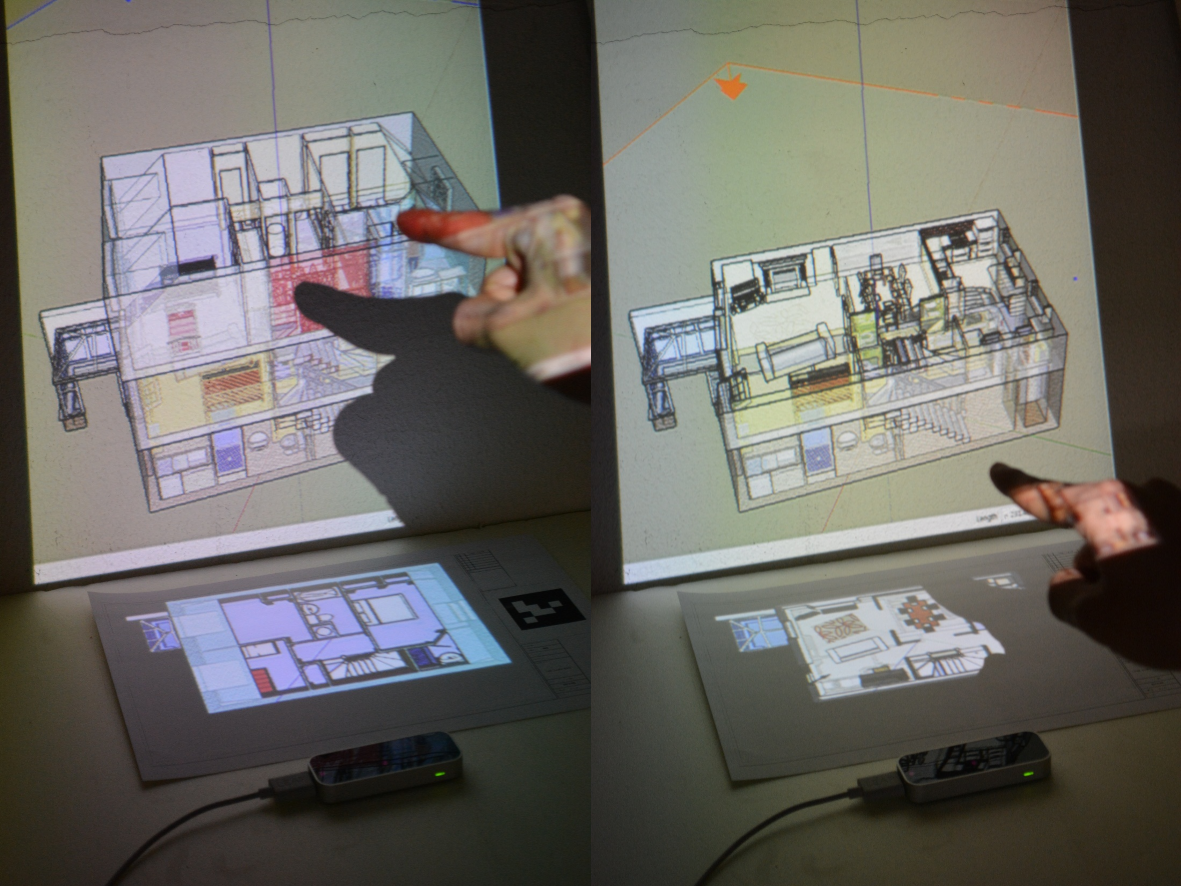
\includegraphics[width=0.9\columnwidth]{4-Interaction_Design/query_plane}
\caption{Querying Specific Floor Plan}
\label{fig:layer}
\end{figure}


%%%%%%%%
\subsection{Additional Information Retrieval}
건축 공정 중에 도면의 부가적인 정보를 계산하여야 하는 경우가 빈번하다. 특히 \cite{song_penlight:_2009}에서 제안한 것과 같이 건축 도면에서 부가적인 Dimension 정보를 제공하는 것은 시공 현장에서 유용하게 사용된다. 제안하는 시스템에서는 SketchUp의 Entity 정보를 이용하여 이러한 Dimension 정보를 계산한다. 또한 기존 시스템에서는 2차원 정보만 증강되었던데 반하여 3차원 모델을 in-air에서 터치함으로써 벽면의 넓이나 기둥의 높이 등 3차원 Entity의 Dimension도 제공할 수 있다. \textit{또한, Mobile Personal Workspace에서는 모바일 기기 화면에 있는 컨텐츠를 터치하여 부가적인 정보를 얻을 수 있도록 하였다. 하지만, 손가락으로 터치하는 것이 정밀하지 못하기 때문에 불편하다는 피드백이 많았다. 추후 연구에서는 영역 확대와 같은 기능을 추가하여 인식의 정밀도를 높이는 것이 필요하다.}

\begin{figure*}[!ht]
	\centering
        \begin{subfigure}[b]{0.55\textwidth}
	        \centering
                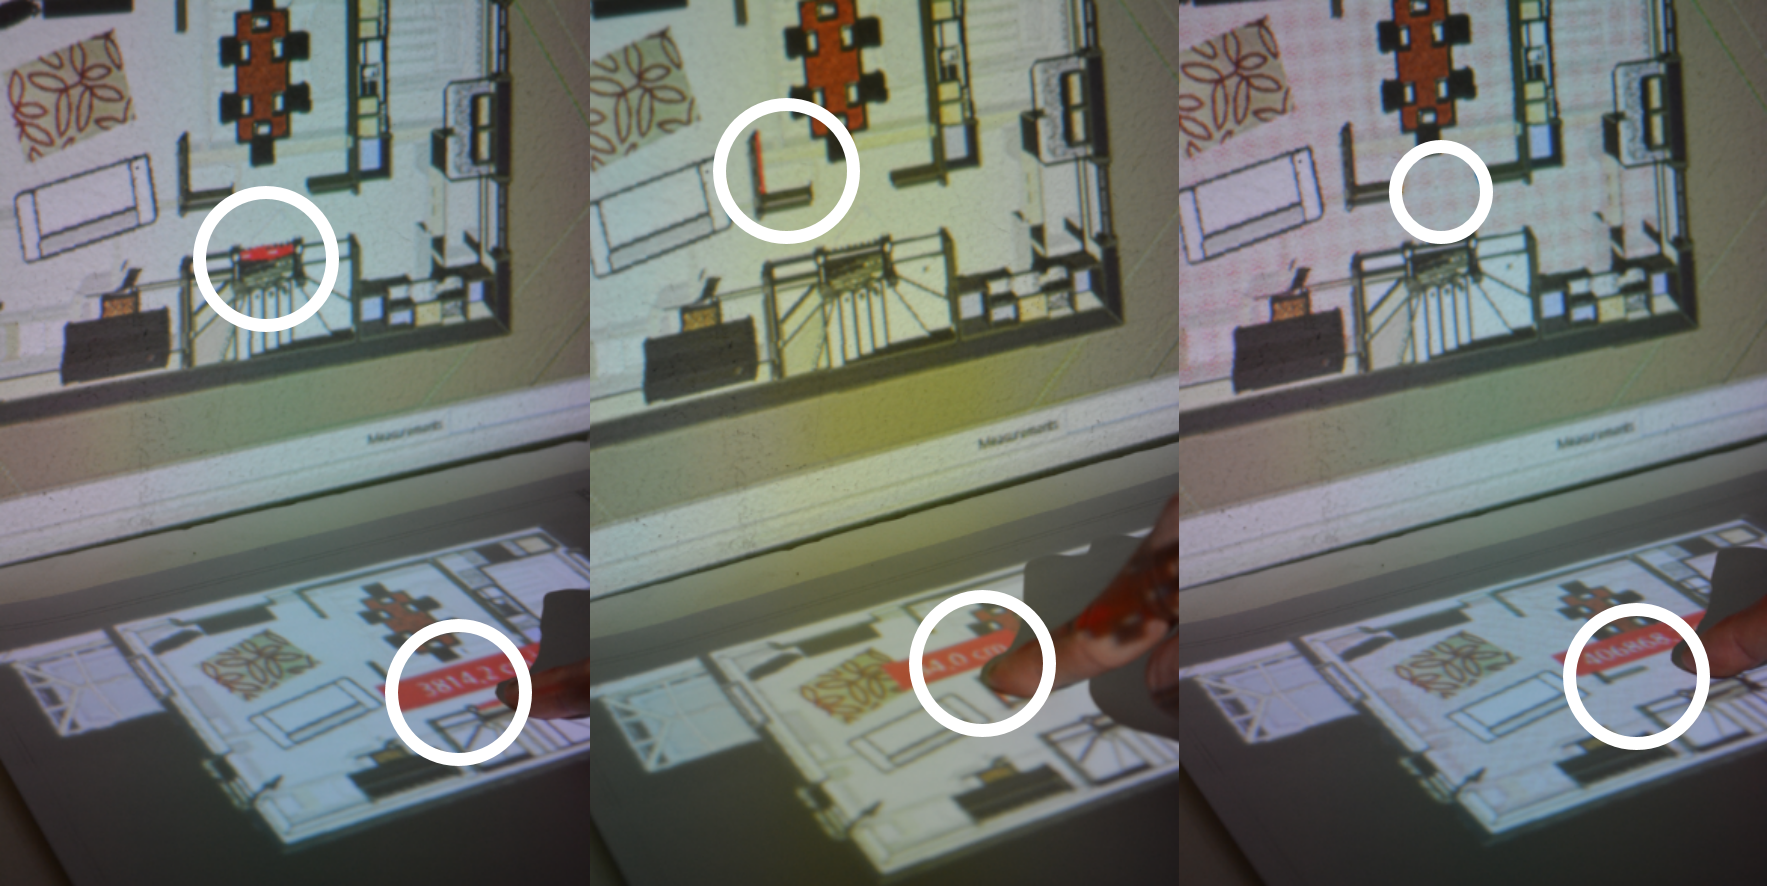
\includegraphics[width=\textwidth]{4-Interaction_Design/2d_info}
                \caption{Querying 2D information - length, area, volumn of specific entity}
                \label{fig:2d_info}
        \end{subfigure}%
        \hfill
        \begin{subfigure}[b]{0.37\textwidth}
            \centering
            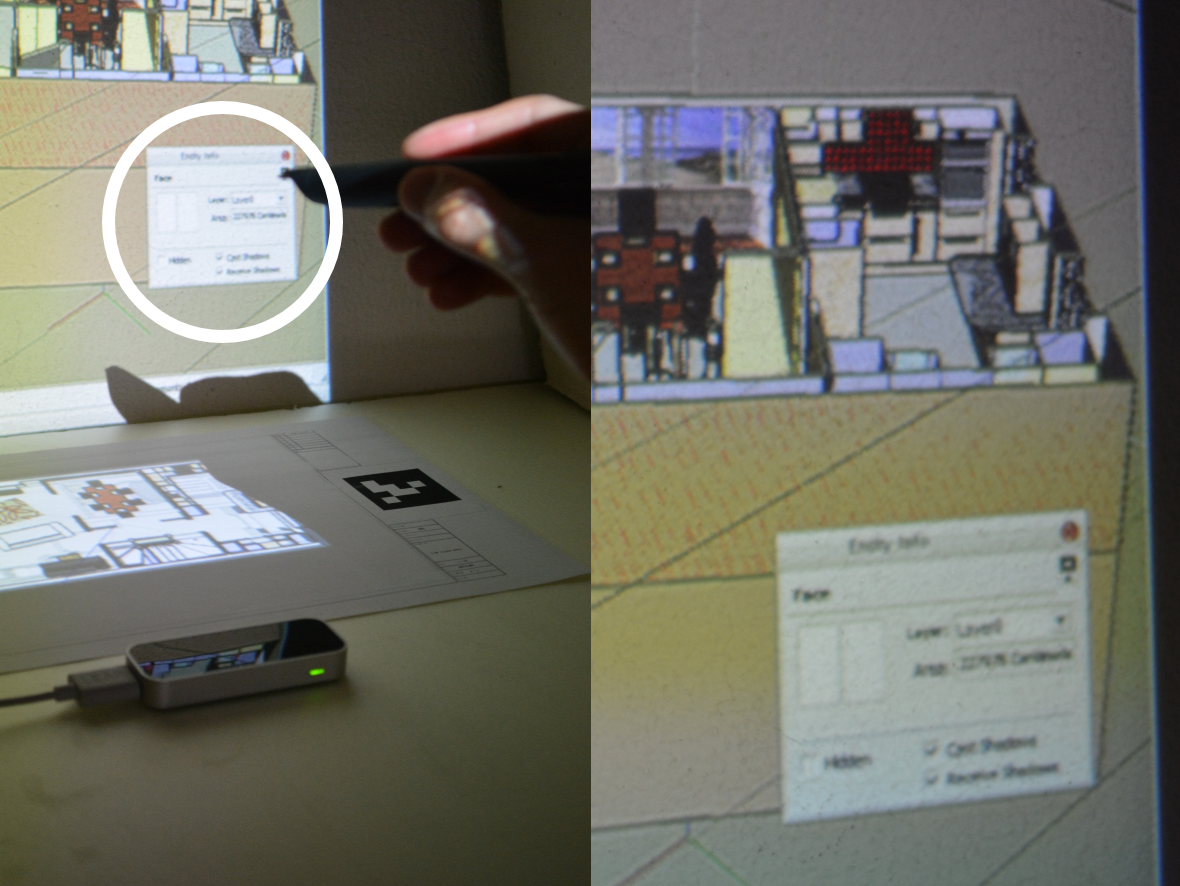
\includegraphics[width=\textwidth]{4-Interaction_Design/3d_info}
                \caption{3D information}
                \label{fig:3d_info}
        \end{subfigure}
	\caption{3D Manipulation}
    \label{fig:infor}
\end{figure*}

\subsubsection{2-Dimensional Information Retrieval}
2차원 정보 제공은 Figure \ref{fig:2d_info}와 같이 도면에 나타난 벽면의 길이(그림 \ref{fig:2d_info} 왼쪽)나 바닥 면(그림 \ref{fig:2d_info} 오른쪽), 가구 등의 부피(그림 \ref{fig:2d_info} 중앙) 등을 도면을 직접 터치함으로써 획득할 수 있다. 이는 해당 건축 도면 상에서 터치된 2차원 좌표를 \textit{SketchUp} 프로그램에 질의하여 \textit{Entity} 정보를 획득하여 보여주게 된다.
\subsubsection{3-Dimensional Information Retrieval}
\textit{3차원 정보 제공은 그림 \ref{fig:3d_info}와 같이 3차원 모델의 \textit{entity}를 선택함으로써 정보를 제공받게 된다. Vertical Screen의 3차원 모델을 선택하기 위해서는 Leap Motion 기반의 손가락 인식 기술을 사용하여 Screen Tap 제스처를 이용하여 입력이 제공된다. Mobile Personal Workspace에서는 3D 모드에서 모델을 선택하여 선택된 위치를 SketchUp에 질의하여 정보를 얻게 된다.}



%%%%%%%%
\subsection{On-site Editing}
\textit{
실제 시공 환경에서는 여러가지 이유로 도면이나 모델의 계획을 벗어나 시공을 수행해야하는 경우들이 발생한다. 현재 시공 환경에서는 건축 정보에 접근과 수정이 어렵기 때문에 이러한 수정 사항들이 도면으로 다시 재반영되어 갱신되지 않는 경우가 많다. 제안하는 시스템에서는 펜이나 터치를 이용하여 기존의 Entity를 선택하고 이를 이동하거나 수정할 수 있도록 하였다. Shared Smart Space 에서는 펜을 이용하고 스케치 인식 기술을 이용하여 수정되어야 하는 내용을 인식하였으며, Mobile Personal Workspace에서는 터치와 Drag를 인식하여 수정사항을 인식하였다.}
 \begin{figure}[h!]
\centering
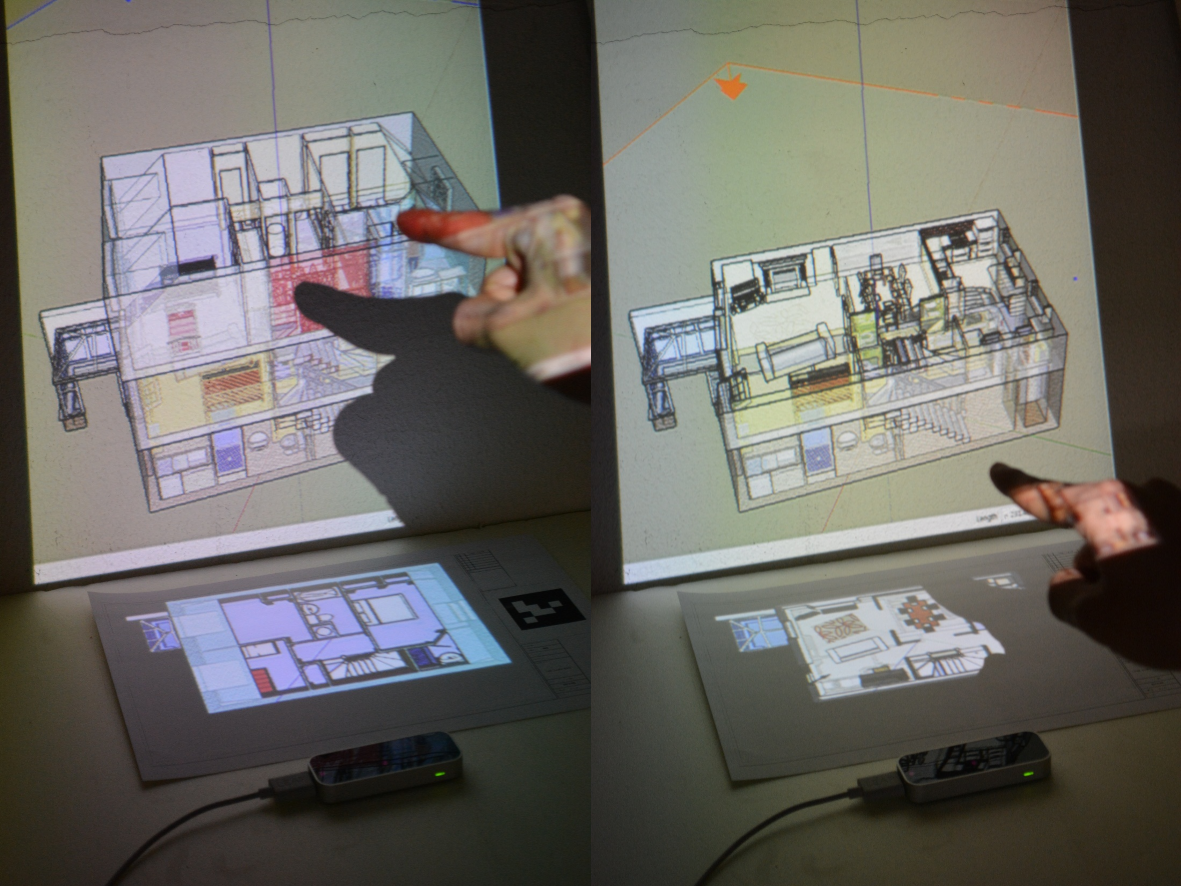
\includegraphics[width=0.9\columnwidth]{4-Interaction_Design/query_plane}
\caption{Querying Specific Floor Plan}
\label{fig:layer}
\end{figure}
